\documentclass{beamer}

\usepackage{amsmath}
\usetheme{default}

\title[Wind Error]{Trading wind power closer to real-time and other multi-market questions.}
\author[J. Mauritzen]{Johannes Mauritzen}
\institute[NHH]{
  Department of Business and Management Science\\
  NHH Norwegian School of Economics\\[1ex]
  jmaurit.github.io\#research\\
  \texttt{johannes.mauritzen@nhh.edu} 
}
\date[Jan 2014]{January 2014}

\begin{document}

%--- the titlepage frame -------------------------%
\begin{frame}[plain]
  \titlepage
\end{frame}


%--- the presentation begins here ----------------%

%--- Intro 						  ----------------%
%--- the presentation begins here ----------------%

\begin{frame}[plain]
	\begin{figure}
	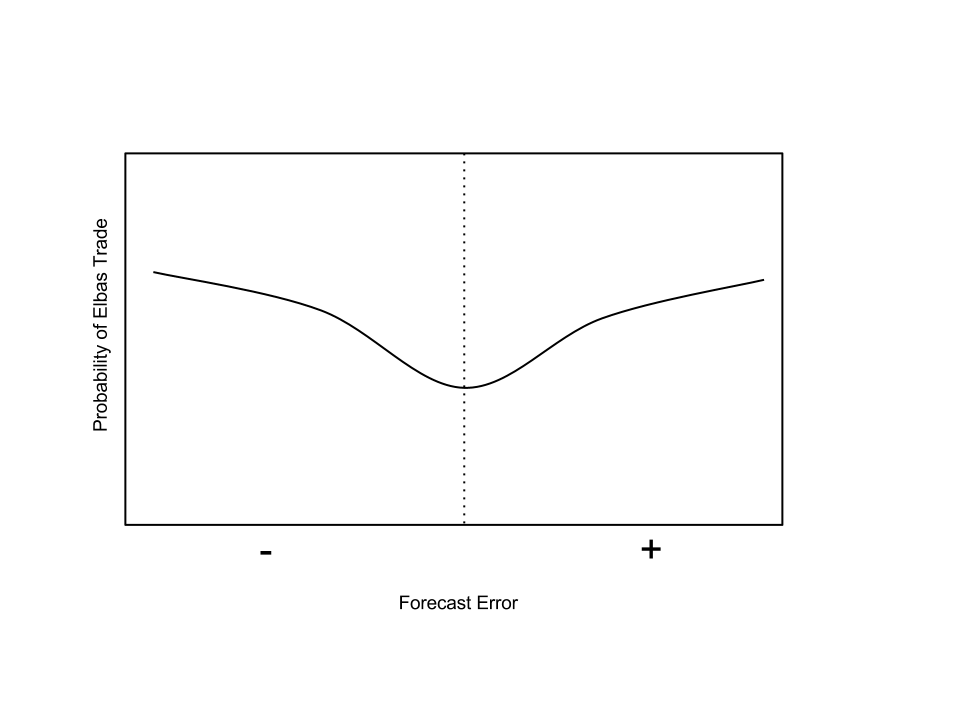
\includegraphics[width=1\textwidth]{figures/ExpectedRelationship.png}
	\end{figure}
\end{frame}

\begin{frame}[plain]
	\begin{figure}
	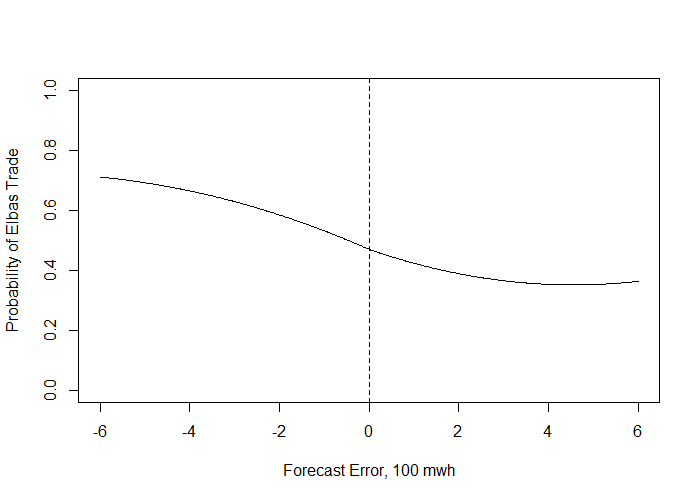
\includegraphics[width=1\textwidth]{figures/FittedQuadratic.png}
	\end{figure}
\end{frame}

\begin{frame}[plain]
	\begin{itemize}
	\item Holttinen (2005) ``Optimal Electricity Market for Wind Power''
	\item Holttinen et al. (2006) ``Prediction Errors and Balancing Costs for Wind Power Production in Finland''
	\
	\end{itemize}
\end{frame}

\begin{frame}[plain]
	\begin{figure}
	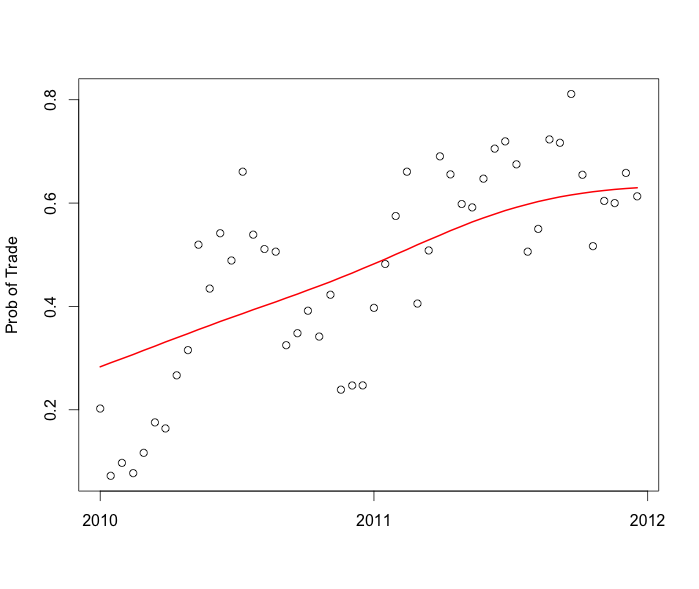
\includegraphics[width=1\textwidth]{figures/ElbTradeOverTime.png}
	\end{figure}
\end{frame}

\begin{frame}[plain]
	\begin{itemize}
	\item Weber (2010) ``Adequate Intraday Market Design to Enable the Integration of Wind Energy into the European Power Systems''
	\end{itemize}
\end{frame}


\begin{frame}[plain]
	\begin{figure}
	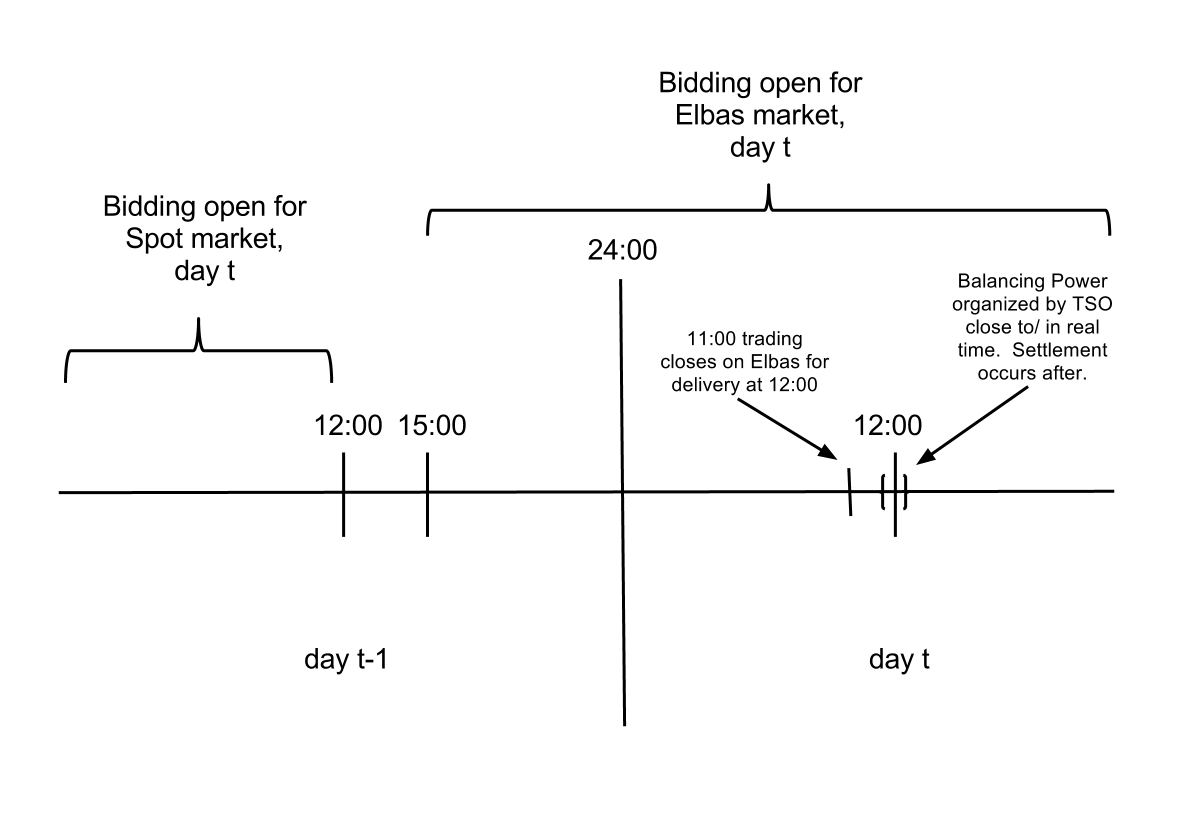
\includegraphics[width=1\textwidth]{figures/MarketTiming.png}
	\end{figure}
\end{frame}

\begin{frame}[plain]
	\begin{figure}
	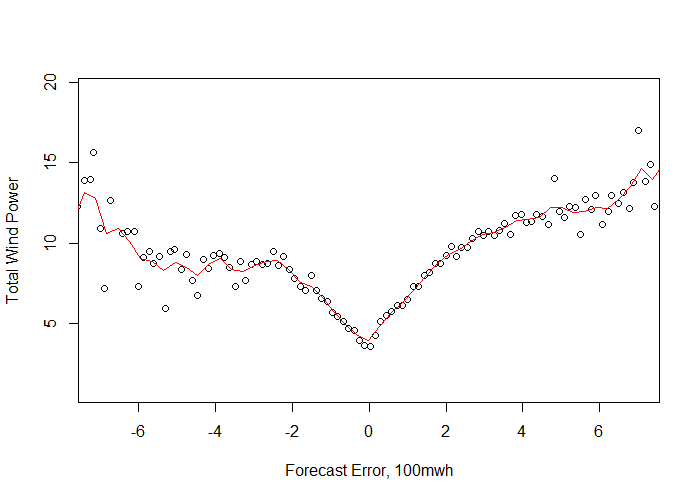
\includegraphics[width=1\textwidth]{figures/windAndForecastError.png}
	\end{figure}
\end{frame}

\begin{frame}[plain]
	\begin{figure}
	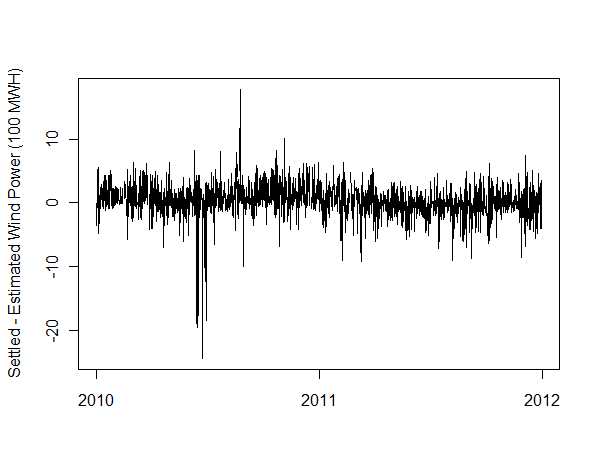
\includegraphics[width=1\textwidth]{figures/Settled-Estimated.png}
	\end{figure}
\end{frame}

\begin{frame}[plain]
	\begin{equation}
		\begin{split}
		Prob_t^{Elbas}&=\alpha + \beta_1 forError_t^{+} + \beta_2 (forError^{+})_t^2 \\
		& \quad + \beta_3 forError_t^-+\beta_4 (forError^-)_t^2 + \epsilon_t    
	\label{glm_eqn}
		\end{split}
	\end{equation}
\end{frame}

\begin{frame}[plain]
	\begin{figure}
	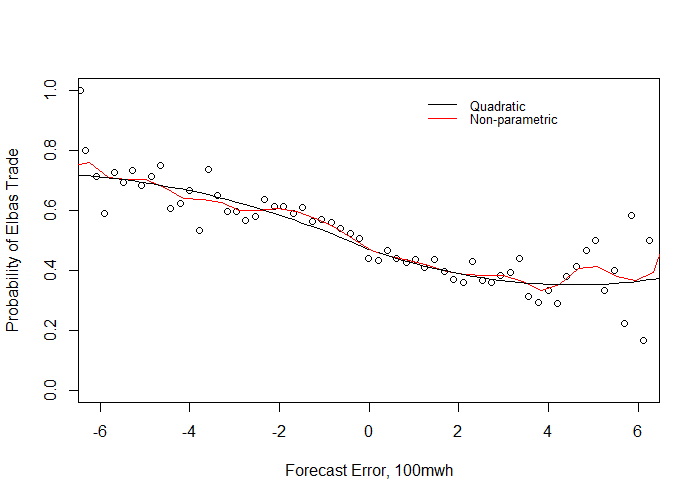
\includegraphics[width=1\textwidth]{figures/Rplot04.png}
	\end{figure}
\end{frame}

\begin{frame}[plain]
	\begin{figure}
	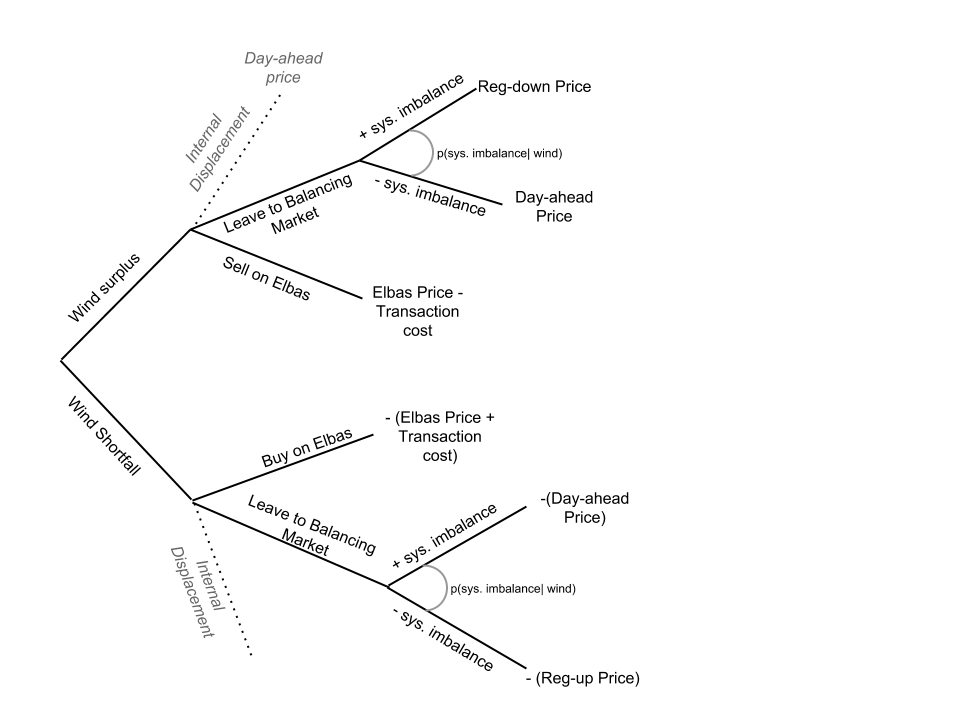
\includegraphics[width=1\textwidth]{figures/DecisionTree.png}
	\end{figure}
\end{frame}

\begin{frame}[plain]
	\begin{figure}
	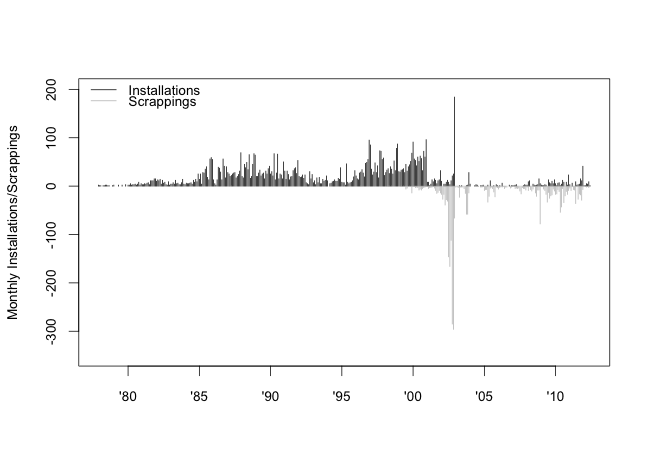
\includegraphics[width=1\textwidth]{figures/turbineInstallations.png}
	\end{figure}
\end{frame}


\begin{frame}[plain]
	\begin{figure}
	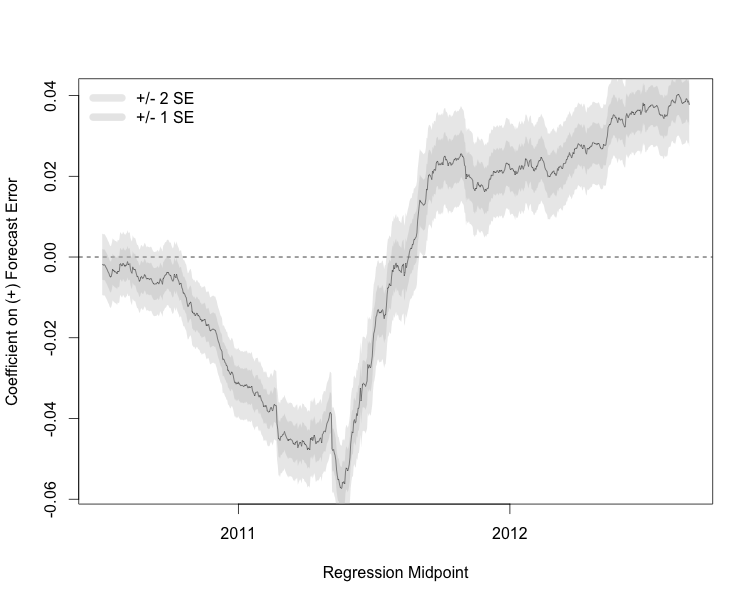
\includegraphics[width=1\textwidth]{figures/WindowRegression.png}
	\end{figure}
\end{frame}


\begin{frame}[plain]
	Trade on Elbas Decision Rule:
		\begin{align}
		 E(\pi_{elbas}) > E(\pi_{balancing})) 
	\label{glm_eqn}
		\end{align}
\end{frame}

\begin{frame}[plain]
	\begin{figure}
	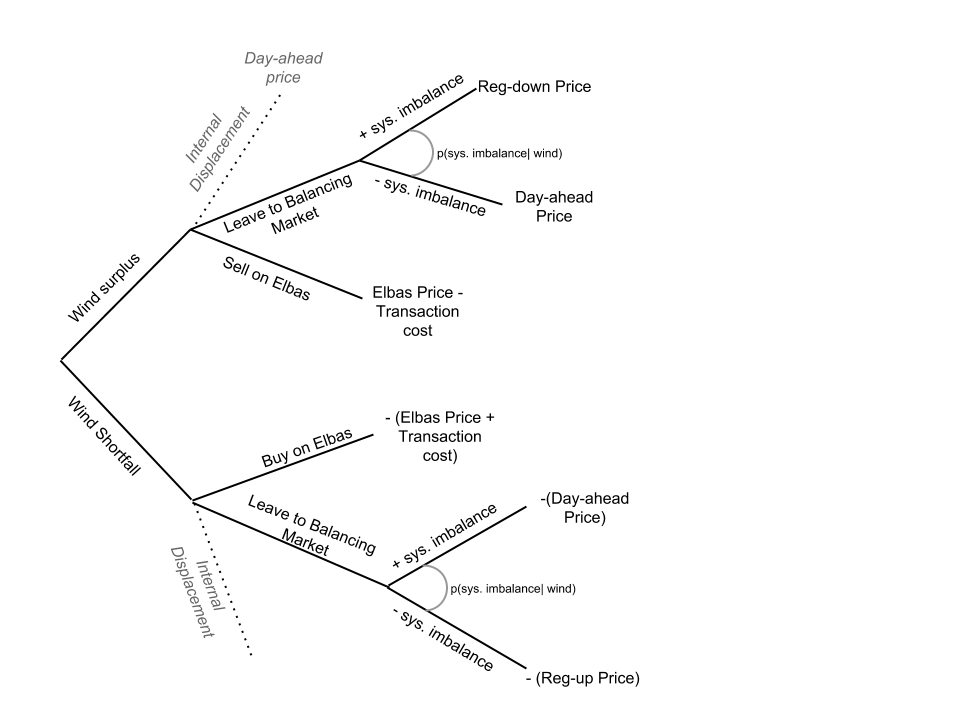
\includegraphics[width=1\textwidth]{figures/DecisionTree.png}
	\end{figure}
\end{frame}

\begin{frame}[plain]
		\begin{align*}
		 pi_{elbas} &= p_{elbas} * q_{imbalance} - t \\
		 pi_{balancing}^{+} &=  \theta*E(P_{regDown})*q_{imbalance}^{+} + (1-\theta)*p_{spot}*q_{imbalance}^{+}\\
		 pi_{balancing}^{-} &= \theta*p_{spot}*q_{imbalance}^{-} + (1-\theta)*E(P_{regUp})*q_{imbalance}^{-}
		\end{align*}
\end{frame}

\begin{frame}[plain]
	Simulated Data (Very Unrealistic!)
		\begin{align*}
		 imbalance_i & \sim N(0, capcity/4)\\
		 p_{spot} & \sim N(30, 10)\\
		 p_{elbas} &= p_{spot} + \epsilon\\
		 p_{regDown} &= p_{spot} - abs(\epsilon) \\
		 p_{regUp} &= p_{spot} + abs(\epsilon) \\
		 \epsilon &\sim N(0,4) \\
		 \Theta = .5
		 t&=0
		\end{align*}
\end{frame}

\begin{frame}[plain]
	\begin{figure}
	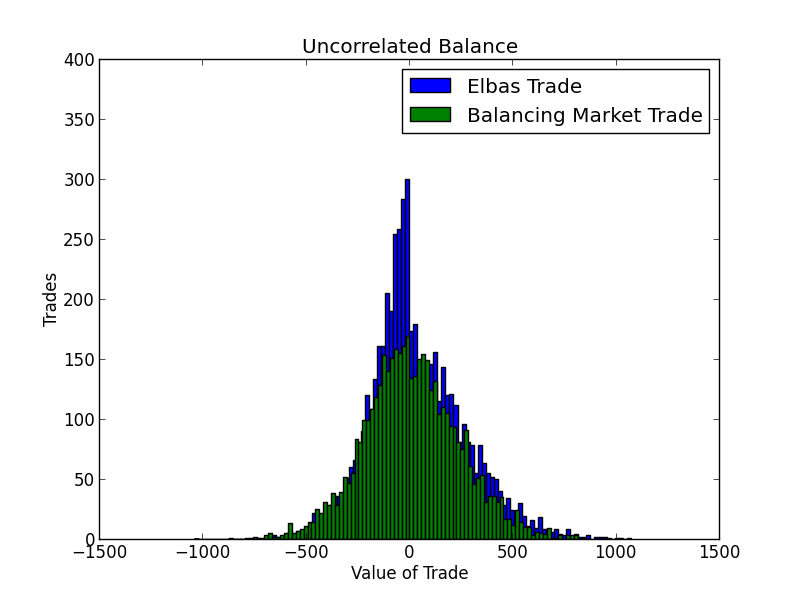
\includegraphics[width=1\textwidth]{figures/elbas_model_a.png}
	\end{figure}
\end{frame}

\begin{frame}[plain]
	Extensions
	\begin{itemize}
	\item $\theta$ (system imbalance) correlated with generator imbalance
	\item Elbas and Regulation Prices Correlated with Wind Power Imbalances
	\end{itemize}
\end{frame}

\begin{frame}[plain]
	\begin{figure}
	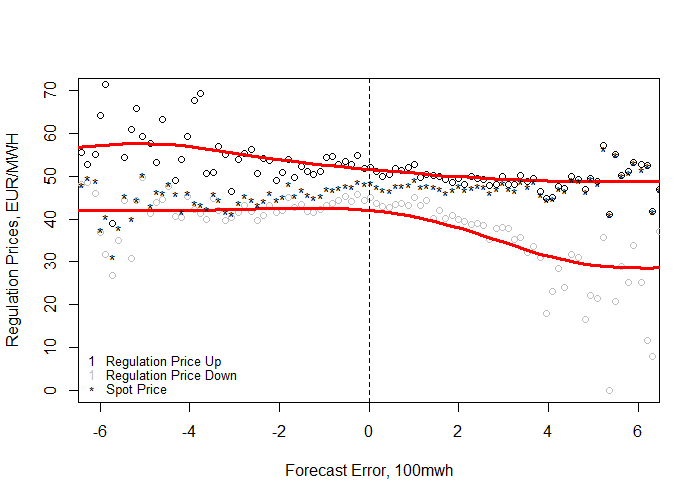
\includegraphics[width=1\textwidth]{figures/RegulationPrices.png}
	\end{figure}
\end{frame}

\begin{frame}[plain]
	Extensions
	\begin{itemize}
	\item $\theta$ (system imbalance) correlated with generator imbalance
	\item Elbas and regulation prices correlated with wind power imbalances
	\item Strategic interactions
	\end{itemize}
\end{frame}


\end{document}